%zCh7_App.tex
%Add sigs to tables
    % \item \nonS \i{p} $>$ .1, \marS \i{p} $<$ .1, \oneS \i{p} $<$ .05, \twoS \i{p} $<$ .01, \thrS \i{p} $<$ .001. 

\section{Appendix}
    \subsection{Subject means statistical analyses}
        % What is
            The following section includes more traditional ANOVAs and t-tests than are included in the main body of this work. This section is not intended to be interpreted as scientific findings, but instead serves as a basis of comparison for more nuanced mixed effects models. The broad lesson that can be gleaned from the statistics presented below is that, with the exception of Model effects from Experiment 1, all findings are sufficiently robust as to be seen when taking individual subject means. Random effects components of the first mixed model of Experiment 1 appear to be required to highlight the subtle effects described. \par 
        \subsubsection{Experiment 1: Shadowing, Egocentric Bias}
                \begin{table}[!h]\centering \begin{threeparttable} 
                    \caption[Shadowing effect of Model ANOVA]{Mixed, repeated measures ANOVA analysis for Shadowing effect of Model, stimulus Type, and Group.} \label{tab:anova_shad_ego}
                    \begin{tabular}{lScSSS}
                    \toprule  
                    \multicolumn{1}{c}{Source} & \multicolumn{1}{c}{\i{SS}} &
                    \multicolumn{1}{c}{\i{df}} & \multicolumn{1}{c}{\i{MS}} &
                    \multicolumn{1}{c}{\i{F}} & \multicolumn{1}{c}{\i{p}} 
                    \\ \midrule 
                        \multicolumn{6}{l}{Within-Subjects} \\
                        \IE Type & 2541.242 & 1 & 2541.242 & 0.41 & 0.526\\
                        \IE Type * Group & 16886.771 & 1 & 16886.771 & 2.724 & 0.108\\
                        \IE Error(Type) & 223191.724 & 36 & 6199.77 &  & \\
                        \IE Model & 1958.251 & 1 & 1958.251 & 0.95 & 0.336\\
                        \IE Model * Group & 2452.365 & 1 & 2452.365 & 1.19 & 0.283\\
                        \IE Error(Model) & 74195.436 & 36 & 2060.984 &  & \\
                        \IE Type * Model & 6218.873 & 1 & 6218.873 & 6.843 & 0.013\\
                        \IE Type * Model * Group & 141.777 & 1 & 141.777 & 0.156 & 0.695\\
                        \IE Error(Type*Model) & 32716.09 & 36 & 908.78 &  & \\
                        \multicolumn{6}{l}{Between-Subjects} \\
                        \IE Group & 3993.3 & 1 & 3993.3 & 0.076 & 0.784\\
                        \IE Error & 1892301.824 & 36 & 52563.94 &  & \\
                    \bottomrule \end{tabular} \begin{tablenotes}
                        \small
                          \item \i{Note}. \i{SS} = Type III Sum of Squares; \i{df} = degrees of freedom; \i{MS} = mean square; \i{F} = F critical value; \i{p} = p-value significance. Model reported as linear effect across three levels.
                    \end{tablenotes} \end{threeparttable} \end{table} 
                \begin{table}[!h]\centering \begin{threeparttable} 
                    \caption[Shadowing effect of Model t-tests]{Follow-up two-tailed t-tests for Shadowing effect of Model, across Group and stimulus Type.} \label{tab:tstat_shad_ego}
                    \begin{tabular}{lSSScS}
                    \toprule  
                    \multicolumn{1}{c}{Source} & 
                    \multicolumn{1}{c}{\i{M}} & \multicolumn{1}{c}{\i{SD}} & 
                    \multicolumn{1}{c}{\i{t}} & \multicolumn{1}{c}{\i{df}} & \multicolumn{1}{c}{\i{p}} 
                    \\ \midrule
                    \multicolumn{6}{l}{Signers} \\
                    \multicolumn{6}{l}{\IE Grooming Gesture} \\
                    \IE\IE Self vs. Friend  & -9.603 & 38.299 & -1.121 & 19 & 0.276\\
                    \IE\IE Friend vs. Other  & -4.286 & 43.136 & -0.444 & 19 & 0.662\\
                    \multicolumn{6}{l}{\IE Pseudosigns} \\
                    \IE\IE Self vs. Friend  & -13.279 & 71.606 & -0.829 & 19 & 0.417\\
                    \IE\IE Friend vs. Other & 28.88 & 55.252 & 2.338 & 19 & 0.031\\
                    \multicolumn{6}{l}{Nonigners} \\
                    \multicolumn{6}{l}{\IE Grooming Gesture} \\
                    \IE\IE Self vs. Friend  & -21.029 & 71.058 & -1.29 & 18 & 0.213\\
                    \IE\IE Friend vs. Other  & -5.896 & 74.98 & -0.334 & 17 & 0.743\\
                    \multicolumn{6}{l}{\IE Pseudosigns} \\
                    \IE\IE Self vs. Friend  & -4.233 & 89.563 & -0.206 & 18 & 0.839\\
                    \IE\IE Friend vs. Other & 3.776 & 80.058 & 0.2 & 17 & 0.844\\
                    \bottomrule
                    \end{tabular}
                    \begin{tablenotes}
                        \small
                          \item \i{Note}. \i{M} = Mean; \i{SD} = Standard Deviation; \i{t} = t-test value; \i{df} = degrees of freedom;  \i{p} = p-value significance. Self vs. Friend reflects Egocentric Bias. Friend vs. Other reflects effect of Visual Familiarity.
                    \end{tablenotes} \end{threeparttable} \end{table} 
        \clearpage
        \subsubsection{Experiment 1: Shadowing, Symmetricity}
                \begin{table}[!h]\centering \begin{threeparttable} 
                    \caption[Shadowing effect of Symmetricity ANOVA]{Mixed, repeated measures ANOVA analysis for Shadowing effect of Symmetricity (Sym), stimulus Type, and Group.} \label{tab:anova_shad_sym}
                    \begin{tabular}{lScSSr}
                    \toprule  
                    \multicolumn{1}{c}{Source} & \multicolumn{1}{c}{\i{SS}} &
                    \multicolumn{1}{c}{\i{df}} & \multicolumn{1}{c}{\i{MS}} &
                    \multicolumn{1}{c}{\i{F}} & \multicolumn{1}{c}{\i{p}} 
                    \\ \midrule 
                        \multicolumn{6}{l}{Within-Subjects} \\
                        \IE Type & 474.509 & 1 & 474.509 & 0.108 & 0.745\\
                        \IE Type * Group & 15985.255 & 1 & 15985.255 & 3.628 & 0.065\\
                        \IE Error(Type) & 163034.927 & 37 & 4406.349 &  & \\
                        \IE Sym & 4254.106 & 1 & 4254.106 & 8.841 & 0.005\\
                        \IE Sym * Group & 500.871 & 1 & 500.871 & 1.041 & 0.314\\
                        \IE Error(Sym) & 17804.540 & 37 & 481.204 &  & \\
                        \IE Type * Sym & 5542.043 & 1 & 5542.043 & 20.629 & $<$ .001\\
                        \IE Type * Sym * Group & 2176.249 & 1 & 2176.249 & 8.101 & 0.007\\
                        \IE Error(Type*Sym) & 9939.921 & 37 & 268.647 &  & \\
                        \multicolumn{6}{l}{Between-Subjects} \\
                        \IE Group & 4870.890 & 1 & 4870.890 & 0.142 & 0.709\\
                        \IE Error & 1271300.290 & 37 & 34359.467 &  & \\
                    \bottomrule \end{tabular} \begin{tablenotes}
                        \small
                          \item \i{Note}. Sym = Symmetricity; \i{SS} = Type III Sum of Squares; \i{df} = degrees of freedom; \i{MS} = mean square; \i{F} = F critical value; \i{p} = p-value significance. 
                    \end{tablenotes} \end{threeparttable} \end{table}
                \begin{table}[!h]\centering \begin{threeparttable} 
                    \caption[Shadowing effect of Symmetricity t-tests]{Follow-up two-tailed t-tests for Shadowing effect of Symmetricity, across Group and stimulus Type.} \label{tab:tstat_shad_sym}
                    \begin{tabular}{lSSScS}
                    \toprule  
                    \multicolumn{1}{c}{Source} & 
                    \multicolumn{1}{c}{\i{M}} & \multicolumn{1}{c}{\i{SD}} & 
                    \multicolumn{1}{c}{\i{t}} & \multicolumn{1}{c}{\i{df}} & \multicolumn{1}{c}{\i{p}} 
                    \\ \midrule
                    \multicolumn{6}{l}{Signers} \\
                    \IE Gest: Asym-Sym & 9.580 & 22.400 & 1.913 & 19 & 0.071\\
                    \IE PSign: Asym-Sym & 18.485 & 27.584 & 2.997 & 19 & 0.007\\
                    \multicolumn{6}{l}{Nonigners} \\
                    \IE Gest: Asym-Sym & -12.534 & 30.18 & -1.810 & 18 & 0.087\\
                    \IE PSign: Asym-Sym & 26.260 & 28.968 & 3.951 & 18 & 0.001\\
                    \bottomrule
                    \end{tabular}
                    \begin{tablenotes}
                        \small
                          \item \i{Note}. Gest = Grooming Gesture; PSign = Pseudosign; Asym = Asymmetrical; Sym = Symmetrical; \i{M} = Mean; \i{SD} = Standard Deviation; \i{t} = t-test value; \i{df} = degrees of freedom;  \i{p} = p-value significance.
                    \end{tablenotes} \end{threeparttable} \end{table} 
        \clearpage
        \subsubsection{Experiment 2: Transition, Condition}
                \begin{table}[!h]\centering \begin{threeparttable} 
                    \caption[Transitions effect of Condition ANOVA]{Mixed, repeated measures ANOVA analysis for Transitions effect of Condition (Cond), stimulus Type, and Group.} \label{tab:anova_trans_cond}
                    \begin{tabular}{lScSSr}
                    \toprule  
                    \multicolumn{1}{c}{Source} & \multicolumn{1}{c}{\i{SS}} &
                    \multicolumn{1}{c}{\i{df}} & \multicolumn{1}{c}{\i{MS}} &
                    \multicolumn{1}{c}{\i{F}} & \multicolumn{1}{c}{\i{p}} 
                    \\ \midrule 
                        \multicolumn{6}{l}{Within-Subjects} \\
                        \IE Type & 32293.746 & 1 & 32293.746 & 6.267 & 0.016\\
                        \IE Type * Group & 16132.626 & 1 & 16132.626 & 3.131 & 0.084\\
                        \IE Error(Type) & 206117.357 & 40 & 5152.934 &  & \\
                        \IE Cond & 1271616.482 & 1 & 1271616.482 & 299.196 & $<$ 0.001\\
                        \IE Cond * Group & 7663.748 & 1 & 7663.748 & 1.803 & 0.187\\
                        \IE Error(Cond) & 170004.323 & 40 & 4250.108 &  & \\
                        \IE Type * Cond & 10164.552 & 1 & 10164.552 & 1.741 & 0.195\\
                        \IE Type * Cond * Group & 2033.146 & 1 & 2033.146 & 0.348 & 0.558\\
                        \IE Error(Type*Cond) & 233524.161 & 40 & 5838.104 &  & \\
                        \multicolumn{6}{l}{Between-Subjects} \\
                        \IE Group & 63212.030 & 1 & 63212.030 & 0.837 & 0.366\\
                        \IE Error & 3019254.833 & 40 & 75481.371 &  & \\
                    \bottomrule \end{tabular} \begin{tablenotes}
                        \small
                          \item \i{Note}. Cond = Condition; \i{SS} = Type III Sum of Squares; \i{df} = degrees of freedom; \i{MS} = mean square; \i{F} = F critical value; \i{p} = p-value significance. 
                          \item Condition reported as linear effect across three levels.
                    \end{tablenotes} \end{threeparttable} \end{table} 
                \begin{table}[!h]\centering \begin{threeparttable} 
                    \caption[Transitions effect of Condition t-tests]{Follow-up two-tailed t-tests for Transitiions effect of Condition, across Group and stimulus Type.} \label{tab:tstat_trans_cond}
                    \begin{tabular}{lSSScr}
                    \toprule  
                    \multicolumn{1}{c}{Source} & 
                    \multicolumn{1}{c}{\i{M}} & \multicolumn{1}{c}{\i{SD}} & 
                    \multicolumn{1}{c}{\i{t}} & \multicolumn{1}{c}{\i{df}} & \multicolumn{1}{c}{\i{p}} 
                    \\ \midrule
                        \multicolumn{6}{l}{Signers} \\
                        \multicolumn{6}{l}{\IE Grooming Gesture} \\
                        \IE\IE Normal vs. Blur & -19.192 & 40.978 & -2.146 & 20 & 0.044\\
                        \IE\IE Blur vs. Hold & -145.803 & 46.620 & -14.332 & 20 & $<$ 0.001\\
                        \multicolumn{6}{l}{\IE Pseudosigns} \\
                        \IE\IE Normal vs. Blur & -112.531 & 59.456 & -8.673 & 20 & $<$ 0.001\\
                        \IE\IE Blur vs. Hold & -97.493 & 42.698 & -10.463 & 20 & $<$ 0.001\\
                        \multicolumn{6}{l}{Nonigners} \\
                        \multicolumn{6}{l}{\IE Grooming Gesture} \\
                        \IE\IE Normal vs. Blur & 18.203 & 125.049 & 0.667 & 20 & 0.512\\
                        \IE\IE Blur vs. Hold & -170.097 & 57.455 & -13.567 & 20 & $<$ 0.001\\
                        \multicolumn{6}{l}{\IE Pseudosigns} \\
                        \IE\IE Normal vs. Blur & -40.824 & 107.082 & -1.747 & 20 & 0.096\\
                        \IE\IE Blur vs. Hold & -128.268 & 97.040 & -6.057 & 20 & $<$ 0.001\\
                    \bottomrule
                    \end{tabular}
                    \begin{tablenotes}
                        \small
                          \item \i{Note}. Cond = Condition; \i{M} = Mean; \i{SD} = Standard Deviation; \i{t} = t-test value; \i{df} = degrees of freedom;  \i{p} = p-value significance. Normal vs. Blur reflects attending to handshape change. Blur vs. Hold reflects attending to movement.
                    \end{tablenotes} \end{threeparttable} \end{table} 
        \clearpage
        \subsubsection{Experiment 2: Transitions, Symmetry}
                \begin{table}[!h]\centering \begin{threeparttable} 
                    \caption[Transitions effect of Symmetricity ANOVA]{Mixed, repeated measures ANOVA analysis for Transitions effect of Symmetricity (Sym), stimulus Type, and Group.} \label{tab:anova_shad_sym}
                    \begin{tabular}{lScSSr}
                    \toprule  
                    \multicolumn{1}{c}{Source} & \multicolumn{1}{c}{\i{SS}} &
                    \multicolumn{1}{c}{\i{df}} & \multicolumn{1}{c}{\i{MS}} &
                    \multicolumn{1}{c}{\i{F}} & \multicolumn{1}{c}{\i{p}} 
                    \\ \midrule 
                        \multicolumn{6}{l}{Within-Subjects} \\
                        \IE Type & 22795.122 & 1 & 22795.122 & 6.721 & 0.013\\
                        \IE Type * Group & 12816.537 & 1 & 12816.537 & 3.779 & 0.059\\
                        \IE Error(Type) & 135660.530 & 40 & 3391.513 &  & \\
                        \IE Sym & 264789.044 & 1 & 264789.044 & 139.747 & $<$ 0.001\\
                        \IE Sym * Group & 222.403 & 1 & 222.403 & 0.117 & 0.734\\
                        \IE Error(Sym) & 75791.085 & 40 & 1894.777 &  & \\
                        \IE Type * Sym & 157085.647 & 1 & 157085.647 & 101.667 & $<$ 0.001\\
                        \IE Type * Sym * Group & 16937.954 & 1 & 16937.954 & 10.962 & 0.002\\
                        \IE Error(Type*Sym) & 61803.974 & 40 & 1545.099 &  & \\
                        \multicolumn{6}{l}{Between-Subjects} \\
                        \IE Group & 40587.515 & 1 & 40587.515 & 0.807 & 0.374\\
                        \IE Error & 2010817.002 & 40 & 50270.425 &  & \\
                    \bottomrule \end{tabular} \begin{tablenotes}
                        \small
                          \item \i{Note}. Sym = Symmetricity; \i{SS} = Type III Sum of Squares; \i{df} = degrees of freedom; \i{MS} = mean square; \i{F} = F critical value; \i{p} = p-value significance. 
                    \end{tablenotes} \end{threeparttable} \end{table}
                \begin{table}[!h]\centering \begin{threeparttable} 
                    \caption[Transitions effect of Symmetricity t-tests]{Follow-up two-tailed t-tests for Transitions effect of Symmetricity, across Group and stimulus Type.} \label{tab:tstat_trans_sym}
                    \begin{tabular}{lSSScr}
                    \toprule  
                    \multicolumn{1}{c}{Source} & 
                    \multicolumn{1}{c}{\i{M}} & \multicolumn{1}{c}{\i{SD}} & 
                    \multicolumn{1}{c}{\i{t}} & \multicolumn{1}{c}{\i{df}} & \multicolumn{1}{c}{\i{p}} 
                    \\ \midrule
                    \multicolumn{6}{l}{Signers} \\
                    \IE Gest: Asym-Sym & -122.777 & 44.434 & -12.662 & 20 & $<$ 0.001 \\
                    \IE PSign: Asym-Sym & -40.627 & 49.323 & -3.775 & 20 & 0.001 \\
                    \multicolumn{6}{l}{Nonigners} \\
                    \IE Gest: Asym-Sym & -158.338 & 59.403 & -12.215 & 20 & $<$ 0.001 \\
                    \IE PSign: Asym-Sym & 4.139 & 76.313 & 0.249 & 20 & 0.806 \\
                    \bottomrule
                    \end{tabular}
                    \begin{tablenotes}
                        \small
                          \item \i{Note}. Gest = Grooming Gesture; PSign = Pseudosign; Asym = Asymmetrical; Sym = Symmetrical; \i{M} = Mean; \i{SD} = Standard Deviation; \i{t} = t-test value; \i{df} = degrees of freedom;  \i{p} = p-value significance.
                    \end{tablenotes} \end{threeparttable} \end{table} 
        \clearpage
    \subsection{Stimuli, as described in Table \ref{tab:stim}, with images} \label{sec:stim_app}
        %% OLD Tab Stim App .075
  \newcommand{\graphix}[1]{\includegraphics[scale=.144]{zImgs/zStim_#1.png}}
  \begin{center}
  % \begin{table}[h] %\footnotesize 
  
  % \begin{threeparttable}
  % headerfooter
    \tablefirsthead{%
    \hline
    \multicolumn{2}{c}{Grooming Gestures} & \multicolumn{2}{c}{Pseudosigns} 
      \\ \hline \noalign{\vskip 2mm}
      }
    \tablehead{%
    \noalign{\vskip 1.2in}
    \hline
    \multicolumn{4}{l}{\small\sl continued from previous page}\\
    \hline
    \multicolumn{2}{c}{Grooming Gestures} & \multicolumn{2}{c}{Pseudosigns} 
      \\ \hline \noalign{\vskip 2mm}
      }
    \tabletail{%
    \hline
    \multicolumn{4}{r}{\small\sl continued on next page}\\
    \hline}
    \tablelasttail{\hline}
    \topcaption[Experimental items with Screencaptures]{\normalsize Experimental items for Shadowing, Transitions and Working Memory tasks, with screencaptures highlighting handshape and location. Capitalized glosses indicate phonologically closest existing ASL sign.} \label{tab:stim_app}

    \centering  
    \begin{supertabular*}{\textwidth}{cccc} \hline \shrinkheight{4.5in}
    

     1.  Tug ear  & 7.  Push sleeves  & 1.     BACON & 7.    WHATEVER \\  
    \graphix{G01} & \graphix{G07} & \graphix{S01} & \graphix{S07} \\
    
     2.  Wipe eye  & 8.  Rub Face  & 2.    PERIOD & 8.    BELT \\
    \graphix{G02} & \graphix{G08} & \graphix{S02} & \graphix{S08} \\

     3.  Scratch face  & 9.  Wipe eyes  & 3.    ISREAL & 9.    BEAR \\
    \graphix{G03} & \graphix{G09} & \graphix{S03} & \graphix{S09} \\

     4.  Scratch head  & 10. Stretch arms  & 4.    DRUNK & 10.   LICENSE \\
    \graphix{G04} & \graphix{G10} & \graphix{S04} & \graphix{S10} \\

     5.  Rub nose  & 11. Twiddle  & 5.    GREEN & 11. TEXTING \\
    \graphix{G05} & \graphix{G11} & \graphix{S05} & \graphix{S11} \\
    
     6.  Scratch nose  & 12. Fold Arms     & 6.    BORED & 12.   BYCICLE \\
    \graphix{G06} & \graphix{G12} & \graphix{S06} & \graphix{S12} \\
      \hline \end{supertabular*} 
      % \begin{tablenotes}
      %     \small \item %\i{Note}.
      % \end{tablenotes}
  % \end{threeparttable} 
  % \end{table} 
  \end{center} 
        %\footnote{replace table}
        \clearpage
    \subsection{Example TAMI-h response items}
        \label{sec:tami_example}
        \newcommand{\tamiscale}{.2655}
        \begin{figure}[h] \centering 
            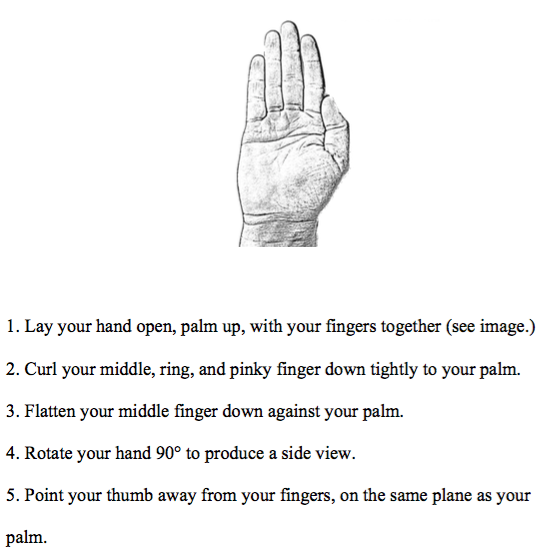
\includegraphics[scale=\tamiscale]{TAMI_1Q}
            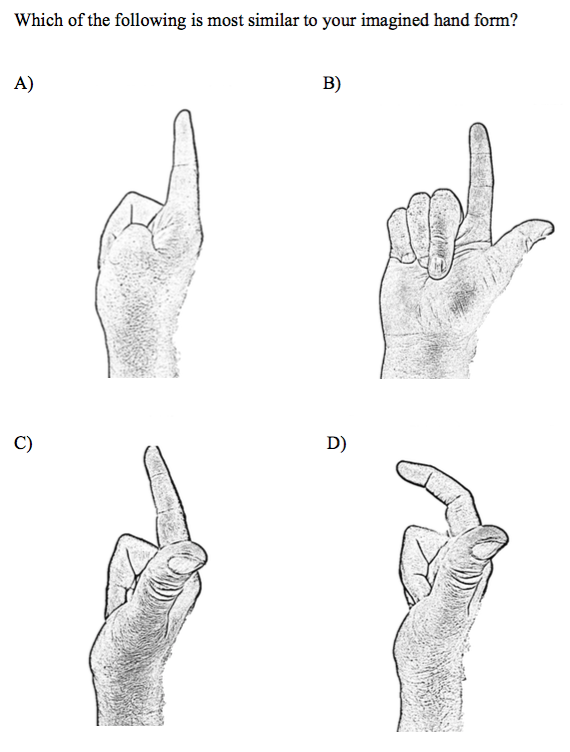
\includegraphics[scale=\tamiscale]{TAMI_1R} \\
            Example trial (left) and Isolated response set (right) \\~\\
            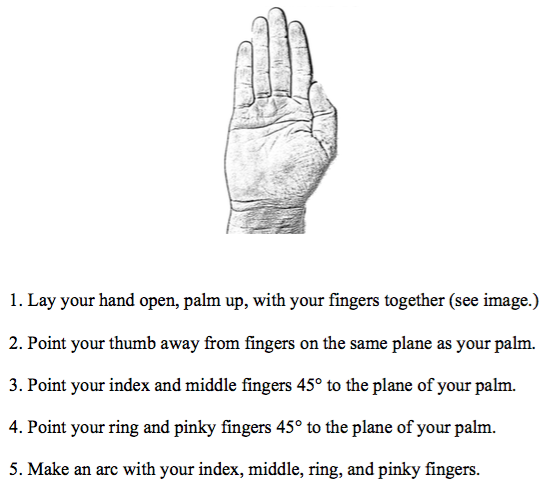
\includegraphics[scale=\tamiscale]{TAMI_2Q}
            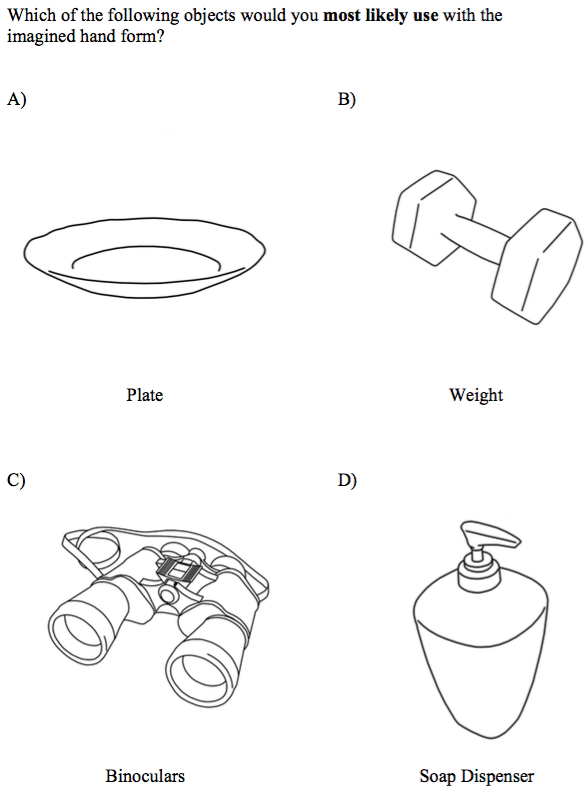
\includegraphics[scale=\tamiscale]{TAMI_2R} \\  
            Example trial (left) and Functional response set (right) \\
            \caption[Example TAMI-h response items]{Example questions and response sets for the Test of Ability in Movement Imagery for hands (TAMI-h): Isolated and Functional substests. See \citeA{donoff2018} for full task description.} \label{fig:tami_example}
        \end{figure} 
    %Near-zero parameter estimates don't produce StdErr
        % https://www.statalist.org/forums/forum/general-stata-discussion/general/1369209-mixed-effects-standard-errors-calculation-failed
        % took out slopes to get SE for subj intercept in TranSym model
            % mixed rt i.group##i.sym##i.type || subj: || item: || place:, reml res(exc) cov(ind) noconstant
    %Made tables with zStata_TableFormatting.xls [ ]{2,}
        % I chose not to publish that xls to github
        % but would send it to you if you emailed me
%%REF
    %\fi
    %\nocite{*}
    \newpage
    \singlespacing 
    % \setlength{\itemsep}{\baselineskip}
    \bibliographystyle{apacite}
    \bibliography{Diss_Ref}